
\documentclass[10pt, journal, compsocconf,a4paper]{IEEEtran}

\usepackage[pdftex]{graphicx}

% correct bad hyphenation here
\hyphenation{op-tical net-works semi-conduc-tor}


\begin{document}
\title{Extending Mocapy++ with a mixed probability distribution\\Advanced Topics In Data Modeling}

\author{\IEEEauthorblockN{Kasper Nybo Hansen}
\IEEEauthorblockA{Dept. of Computer Science\\
University of Copenhagen\\
Copenhagen, Denmark\\
nybo@diku.dk}
}

% make the title area
\maketitle

\begin{abstract}
Mocapy++ is a C++ toolkit for learning and inference in dynamic Bayesian networks. This report describes the implementation, testing and results of extending Mocapy++ with a new node. 

The new node is a mixed node, allowing both discrete and continuous values. The continuous part of the node is a gaussian distribution. The new node is used to calculate a probabilistic model of hydrogen bonding in protein structures. The probabilistic model is learned from a provided dataset.
\end{abstract}

\begin{IEEEkeywords}
Mocapy++; DIKU; Dynamic Bayesian networks; Mixed probability distribution
\end{IEEEkeywords}


\section{Introduction} % (fold)
\label{sec:introduction}

% http://www.stat.uiowa.edu/~nshyamal/22S175/DI.pdf
% 
% http://www.tutorvista.com/math/mixed-probability-distribution
% http://www.freemathhelp.com/forum/viewtopic.php?f=12&t=34692
% 
% Good explanation
% http://www.ds.unifi.it/VL/VL_EN/dist/dist3.html

An introduction with a short discussion of the theory of inference and learning in Bayesian networks, relevant to Mocapy++.


\subsection{Dynamic Bayesian Network} % (fold)
\label{sub:dynamic_bayesian_network}
A Bayesian network consists of a Directed Acyclic Graph where the nodes are random variables. Each edge in a Bayesian network represents a probabilistic dependency. More precisely figure \ref{fig2} shows a Bayesian network where the probability of observing $o1$ is dependent on $h1$. We call the node $o1$ the observed node and $h1$ and $h2$ the hidden nodes. 

\begin{figure}[ht]
\centering
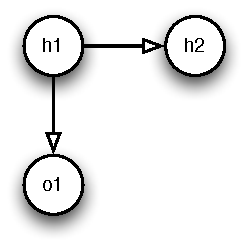
\includegraphics[width=0.1\textwidth]{figures/fig2.pdf}
\caption{Example of the bayesian network}
\label{fig2}
\end{figure}
% subsection dynamic_bayesian_network (end)

\subsection{Mixed node} % (fold)
\label{sub:mixed_node}
The implemented mixed node takes exactly one discrete parent. The parent node can have any size $n$, i.e. it can take on integer values in the range $[0,n]$.
% subsection mixed_node (end)


\subsection{Mixed distribution} % (fold)
\label{sub:mixed_distribution}
The mixed distribution can be divided into two parts. A discrete and continuous part. Let $X$ be a random variable that takes values in the set $S$. We then define the discrete part as the countable set $D \subseteq S$, and the continuous part as $C \subseteq S$. We define a mixed distribution as a distribution that has the following two probabilities

\begin{center}
  \begin{itemize}
    \item $0 < P(x \in D) < 1$
    \item $P(x \in C) = 0$
  \end{itemize} 
  
\end{center}

The discrete part of the distribution can be described by a distribution table. The table will in the implemented node consist of two entries, that sums to exactly $1$. The first entry describes the probability of the node being a discrete node, the second entry describing the probability of the node being a continuous node. Define $P(X = discrete)$ as the probability that the node is discrete, and $1-P(X = discrete)$ as the probability that the node is continuous. 

The continuous part of the mixed distribution consist of the Gaussian distribution aka. the normal distribution. The Gaussian is defined as

\begin{equation}
f(x;\mu,\sigma) = \frac{1}{\sqrt{2\pi\sigma^2}} e^{ -\frac{(x-\mu)^2}{2\sigma^2} }  
\end{equation}
where $\mu$ is the mean value, and $\sigma$ is the standard deviation.

We wish to estimate the parameters of the discrete and continuous distribution. We can do this by the maximum likelihood method. For the discrete case, the maximum likelihood can be calculated as

\begin{equation}
  \hat{P}(X = discrete) = \frac{\#discrete}{\#total}
  \label{eq3} 
\end{equation}
and
\begin{equation}
  \hat{P}(X = continuous) = 1 - \hat{P}(X = discrete)
\end{equation}
where $\#discrete$ denotes the number of discrete observation and $\#total$ denotes the total number of observations.


When estimating the Gaussian variables $\mu$ and $\sigma$ we use the maximum likelihood function for the Gaussian, i.e.
\begin{equation}
  \ln(\mu, \sigma^2) = -\frac{n}{2}\ln(2\pi) - \frac{n}{2}\ln\sigma^2 - \frac{1}{2\sigma^2}\sum_{i=1}^n (x_i-\mu)^2.
\end{equation}
we wish to maximize this function, so we take the derivative and find the stationary points. Doing this yields
\begin{equation}
  \hat{\mu} = \overline{x} \equiv \frac{1}{n}\sum_{i=1}^n x_i, \qquad \hat{\sigma}^2 = \frac{1}{n} \sum_{i=1}^n (x_i - \overline{x})^2
  \label{eq1}
\end{equation}
so the parameters of the Gaussian distribution can be estimated from the continuous samples by the two equations \ref{eq1}. 


Having the parameters to the distribution models in the mixed model we would also like to be able to calculate the likelihood of a sample belonging to the mixed node. We can calculate this likelihood in the following way. Let the sample consist of two elements $s = {d, e}$. The likelihood of $s$ can then be calculated as
\begin{equation} 
L(s) = 
\left\{
\begin{array}{ll} 
  \hat{P}(discrete) & \mathbf{if } d = 0  \\
  \hat{P}(continuous) \frac{1}{\sqrt{2\pi\hat{\sigma}^2}} e^{ -\frac{(e-\hat{\mu})^2}{2\hat{\sigma}^2} }  & \mathbf{if } d = 1    
  \label{eq6}
\end{array} 
\right. 
\end{equation} 
where $\hat{P}(discrete)$ denotes the estimated probability of observing a discrete node, and likewise $\hat{P}(continuous)$. We multiply the Gaussian with $\hat{P}(continuous)$ in order to normalize the mixed distribution.
% subsection mixed_distribution (end)

% subsection d (end)

\subsection{Applications to Hydrogen bounding} % (fold)
\label{sub:applications_to_hydrogen_bounding}
The mixed distribution applies to hydrogen bonding in the following way. A hydrogen bound has two states:

\begin{itemize}
  \item A bond is present or it is not present
  \item If the bond is present it has an energy associated
\end{itemize}

Under the assumption that the energy of a hydrogen bonding can be modeled by a Gaussian probability distribution we can model a hydrogen bond in the following way. The discrete distribution is modeling the first boolean case, i.e. "Is the bond present or not?". If the bond is present, the Continuous part can be used to to find the energy, $E$, of the bond.

The assumption that the energy is modeled by a Gaussian distribution is somewhat crude. Although simple investigation of the energies present in the supplied dataset, actually indicates that the energy could follow a normal distribution.

% subsection applications_to_hydrogen_bounding (end)


% section introduction (end)

\section{Implementation} % (fold)
\label{sec:implementation}

\subsection{Adding the mixed node} % (fold)
\label{sub:adding_the_mixed_node}
The mixed node is added to the framework, by creating a new node type in \texttt{dbn.h}. The new type defines the name of the density and ESS classes, furthermore it defines the typename, which is called \texttt{mixednode}. Furthermore a nodetype is added to \texttt{node.h}, called mixed.

In order to create new nodes, the \texttt{nodefactory} class is extended with a new method called \texttt{new\_mixed\_node}. The new mixed node takes the following parameters

\begin{itemize}
  \item Size: this is only allowed to be 2, but is present for the sake of future works
  \item Name: used in text output, Optional
  \item Init\_random: Randomly initialize the CPD, Optional
  \item CPD: User specified CPD, Optional
  \item Means: User specified Gaussian means array, Optional
  \item Variance: User specified variance array, Optional
\end{itemize}

In this report we assume that the node size of our mixed node is always $2$, this assumption also has the effect that the Gaussian is in 1D. I have included the node size as an argument in order to make it easy to expand the mixed node to handle multidimensional Gaussian distributions in future versions of the mixed node. 

There are several optional arguments to the \texttt{new\_mixed\_node} method. If nothing is specified in the optional arguments the following default behavior is applied. If nothing is specified in init\_random the node will be initialized with a uniform CPD. If nothing is specified in the means and variance arguments then these are initialized randomly.

The node consist of four files:\texttt{ mixedess.h}, \texttt{mixedess.cpp}, \texttt{mixeddensities.h} and \texttt{mixeddensities.cpp}. All four files resides in the \texttt{mixed} directory of the \texttt{src} folder.

The following sections elaborate on the implementation of the individual parts of the node.

% subsection adding_the_mixed_node (end)

\subsection{ESS - inference} % (fold)
\label{sub:ess}
There are two main steps in the framework. The first step is the \emph{E-step}. The E-step is the inference step, where the values of the hidden nodes are inferred by using the set of samples generated by the sampler. The sampler used in this project is the Gibbs sampler that comes with Mocapy++.

Each time a node is sampled the \textbf{E}xpected \textbf{S}ufficient \textbf{S}tatistics (ESS) class is updated. The ESS class acts as a container where the data neccessary to calculate the nodes parameters are stored. For the mixed node, this means storing the following data:

\begin{itemize}
  \item Number of discrete and continuous observations
  \item The energy stored in a way so the Gaussian model parameters can be calculated
\end{itemize}
the parameters needs to be stored for each value that the parent node can take. I.e the size of the tables stored in the ESS, depends on the size of the parent node.

I have implemented the ESS class in the file \texttt{mixed/mixedess.cpp}. The class is responsible for collection data about the sample points, so they can be used later in the density class. Both tables are stored in the ESS array.

The mixedess class stores two tables for later retrieval in the density class. 

Both tables are populated in the class method \texttt{add\_ptv}. This method takes a vector as input. The vector has the format
\begin{equation}
  \{Parent\ value, Indicator, Energy\}
\end{equation}
and is called \emph{ptv}.


If $Indicator=0$ then we know that the sample is a discrete sample, otherwise it must be a continuous sample.

The first table stores the number of observations of discrete and continuous nodes. It has size equal to the parent size $\times$ node size. The table has a row for each value the parent can take. For each value of the parent the ESS thus stores the number of discrete and the number of continuous nodes. Define the parent with value $i$ as $p_i$, and define the size of the parent node as $n$. Then the following table yields an outline of the first table stored in the ESS
\begin{center}
  \begin{tabular}{c | c | c}
  $p_0$ & \#Discrete obs for $p_0$ & \#Continuous obs for $p_0$ \\
  $p_1$ & \#Discrete obs for $p_1$ & \#Continuous obs for $p_1$ \\
  \vdots & \vdots & \vdots \\
  $p_{n-1}$ & \#Discrete obs for $p_{n-1}$ & \#Continuous obs for $p_{n-1}$ 
  \end{tabular}  
\end{center}
where \# means `number of' and obs is a abbreviation for observations.

The second table stored in the ESS has the size parent size $\times$ node size. For each parent value we store two entities. The first entity is the sum of the energies, and the second is the sum of the squared energies. Define all the energy samples belonging to parent $p_i$ as $E_i$, then for each continuous sample with parent value $p_i$ we sum the energy in one column and the sum the energy squared in the other column. An outline of the table can be seen in the following table
\begin{center}
  \begin{tabular}{c | c | c}
  $p_0$ & $\sum_{\forall e \in E_0} e$ & $\sum_{\forall e \in E_0} e^2$ \\
  $p_0$ & $\sum_{\forall e \in E_1} e$ & $\sum_{\forall e \in E_1} e^2$ \\
  \vdots & \vdots & \vdots \\
  $p_{n-1}$ & $\sum_{\forall e \in E_{n-1}} e$ & $\sum_{\forall e \in E_{n-1}} e^2$ \\
  \end{tabular}  
\end{center}
%subsection ess (end)

\subsection{Densities - parameter estimation} % (fold)
\label{sub:densities}
The second step of the framework is the \emph{M-step}. In the M-step we update the parameters of the model, e.g. updating the CPD.

The density class is implemented in the file \texttt{mixed/mixeddensities.cpp}. 

Parameter estimation is done in the method \texttt{estimate}. The function takes the ess array from the ESS class as argument, and calculates the conditional probability density (CPD), means and variance arrays. The CPD is calculated directly from the array containing the number of discrete and the number of continuous observations. The CPD is thus an array where each row contains the probability of observing a continuous and discrete node when given a parent value. 

The estimated probability of observing a discrete value, $\hat{P}(Discrete)$, is calculated as shown in (\ref{eq3}) 

The outline of the CPD table can be seen in the following table 

\begin{center}
  \begin{tabular}{c | c | c}
  $p_0$ & $\hat{P}(Discrete)$ & $\hat{P}(Continuous)$\\
  $p_1$ & $\hat{P}(Discrete)$ & $\hat{P}(Continuous)$\\
  \vdots & \vdots & \vdots \\
  $p_{n-1}$ & $\hat{P}(Discrete)$ & $\hat{P}(Continuous)$ 
  \end{tabular}  
\end{center}

We can calculate the estimated mean and variance of the Gaussian in the following way. Remember we stored the sum of the energies and the sum of the squared energies in the ess array in the ESS class. Furthermore we stored the number of discrete and continuous observations. In both cases we stored the numbers for each parent value. We can thus calculate the mean for the parent value $i$ as
\begin{equation}
  \hat{\mu}_i = \frac{sum_i}{total_i} 
\end{equation}
where $sum_i$ is the total sum of the energies for the parent value $i$, and $total_i$ is the total number of continuous observations for the parent value $i$. The result is a table with the following structure
\begin{center}
  \begin{tabular}{c | c }
  $p_0$ & $\hat{\mu}_1$ \\
  $p_1$ & $\hat{\mu}_2$ \\
  \vdots & \vdots \\
  $p_{n-1}$ & $\hat{\mu}_{n-1}$  
  \end{tabular}  
\end{center}


The variance can be calculated as shown in (\ref{eq1}). From the ess array we also have the squared sum of the energies. The variance is then calculated as
\begin{equation}
  \hat{\sigma_i}^2 = \frac{sumsquared_i}{total_i} - \hat{\mu_i}^2
\end{equation}

where $sumsquared_i$ is the sum of the squared values cumming from the ess. The resulting variance table looks like
\begin{center}
  \begin{tabular}{c | c }
  $p_0$ & $\hat{\sigma_1}^2$ \\
  $p_1$ & $\hat{\sigma_2}^2$ \\
  \vdots & \vdots \\
  $p_{n-1}$ & $\hat{\sigma_{n-1}}^2$  
  \end{tabular}  
\end{center}


\subsection{Densities - likelihood} % (fold)
\label{sub:densities_likelihood}
The likelihood calculation is done in the method \texttt{get\_lik}. The method takes two variables and returns a double. The first variable is the ptv and the second variable is a boolean value indicating if the result should be logarithmic scaled.

Recall that the ptv is a 3-tuple consisting of the values $\{Parent\ value, Indicator, Energy\}$. As usual we define the parent value as $p_i$. Given the ptv, we wish to answer the question, `How likely is it to see this sample given the current model configuration?'. 

We can answer this question in the following way.  If the indicator is $0$ we return the likelihood of seeing a discrete value. This value can be found by making a lookup in the CPD under the given parent value. 

If the indicator is $1$, we know we are in the continuous case. We thus calculate the likelihood as (\ref{eq6}), i.e.

\begin{equation}
  \hat{P}(continuous) \frac{1}{\sqrt{2\pi\hat{\sigma_i}^2}} e^{ -\frac{(e-\hat{\mu_i})^2}{2\hat{\sigma_i}^2} }
  \label{eq20}
\end{equation}
where $\hat{P}(continuous)$ can be found by making a lookup in the CPD table, and where $\mu_i$ and $\sigma_i$ can be found in the means and variances table by making a lookup under $p_i$.


Due to limited precision, the likelihood can become $0$. This can happen when \ref{eq20} is close to $0$. If this happens and the method is called with the boolean flag set to true, an error will occur because we cannot take the logarithm of 0. To remove this problem, we test if the likelihood is calculated as zero. If it is, we set it to the constant \texttt{\_MIN\_TRANSITION}. This ensures that we always will take the logarithm of a positive number.

% subsection densities_likelihood (end)


\subsection{Densitites - sampling} % (fold)
\label{sub:densitites_sampling}
The sampling is done in the method \texttt{sample}. The method takes one argument, namely a parent value. and returns a tuple of two elements. 

The sampling is done in the following way. A random number $r$ is generated such that $0 < r < 1$. 

A lookup in the CPD for the given parent value is performed, yielding the probability of observing a discrete node. Call this probability the \emph{threshold}. If $r \leq threshold$ then the return value of the \texttt{sample} method is the tuple $<0,0>$. The first element in the tuple is the indicator value, and the second is the energy. This energy is assumed to be zero when discrete values are observed.

If $r > threshold$ then we need to sample from the Gaussian distribution. In order to sample from the Gaussian distribution we use the method \texttt{normal\_multivariate} found in \texttt{utils/random\_data.cpp}. This function requires 5 arguments. The first being the dimension of the Gaussian, the second being the number of samples, the third is the standard deviation, the fourth is the mean and the fifth is the random generator to be used. 

We set the dimension and the number of samples to $1$. From the estimate function we have the means and the variances of each of the parent values. We can thus make a lookup in these arrays and find the mean and variance. In order to calculate the standard deviation we take the square root of the variance. The return value of \texttt{normal\_multivariate} is a vector of samples. In our case we only asked for one sample, so the vector has a length of $1$. Call the generated sample for $s$. We then make the \texttt{sample} function return the tuple $<1, s>$.

% subsection densitites_sampling (end)


% subsection densities (end)
%section implementation (end)

\section{Testing of implementation} % (fold)
\label{sec:testing_of_implementation}

This section describes the testing done to ensure that the implemented mixed node works as supposed. 4 test cases 

A description of some simple tests that show that the implementation is correct. 

\subsection{Test of inference and sampling} % (fold)
\label{sub:test_of_sampling}
In this test we would like to confirm that the samples drawn from the mixed node corresponds to the nodes parameters.

The test in \texttt{examples/hmm\_mixed2.cpp} creates two DBN's. The first network is initialized with randomly picked CPD, mean and variance. After initialization abunch of samples is drawn from the network. These samples is then used to train a second network. 

We expect the two networks to have almost identical parameters, i.e. we expect the second network to be able to learn the parameters of the first network that generated the sample points.

The result of the test is

\begin{verbatim}
to0:
  Node: Mixed, size: 1 2 
  Mixed CPD: 
  [0.476073 0.523927 ]

  Gaussian means: 
  0.476903 
  Gaussian variances: 
  0.20354 
  
  
mo0:
  Node: Mixed, size: 1 2 
  Mixed CPD: 
  [0.47202 0.52798 ]

  Gaussian means: 
  0.476937 
  Gaussian variances: 
  0.203367 
\end{verbatim}
As we can see the two nodes are almost identical, which confirms that the inference is working.

In order to test the samples drawn from the discrete part, i have exported the sampled data, and isolated the indicator values. From these values I have made a histogram. I expect the distribution of the indicator values drawn is close to the randomly picked CPD. The CPD in this case is $[0.476073, 0.523927]$

\begin{figure}[ht]
\centering
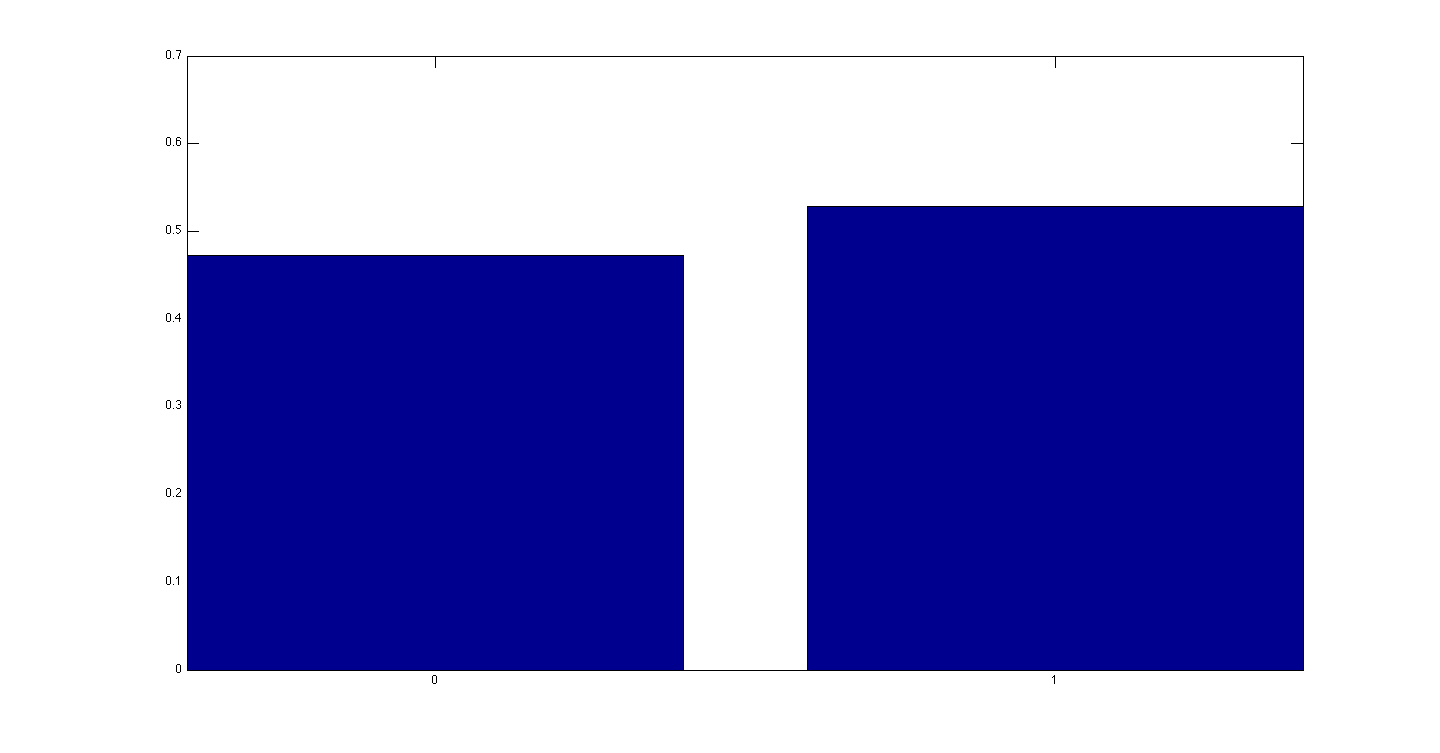
\includegraphics[width=0.5\textwidth]{figures/fig3.png}                                                                             
\caption{Histogram of the indicator values. The distribution of the two, should resemble the randomly generated PCD. The distribution of the drawn indicator values is $[0.47202,  0.52798]$, compared to the randomly picked CPD: $[0.426073, 0.573927]$. There are some discrepancies, but still acceptable.}
\label{fig3}
\end{figure}


In order to show that the sampling is correct, we have extracted the data points generated by the first DBN. The data points consist of both discrete and continuous samples. By isolating the continuous samples, and making a histogram, we expect the histogram to resemble a Gaussian distribution, i.e. take the shape of the bell curve. 

The histogram can be seen on figure \ref{fig1}. On top of the histogram, we have plotted a Gaussian probability density function with the mean and variance equal to the randomly generated. As can be seen from the figure \ref{fig1} the histogram approximates the Gaussian very well, and the conclusion must be that the samples drawn from the continuous part of the distribution is correct.

\begin{figure}
\centering
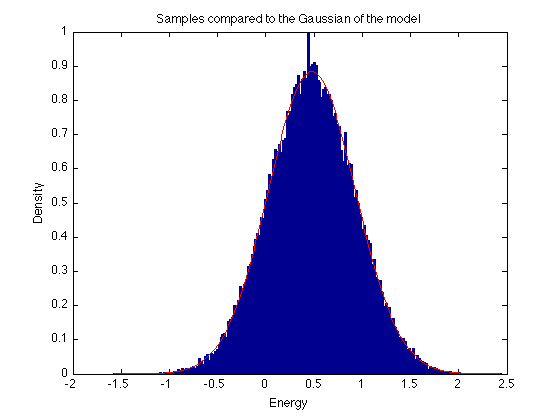
\includegraphics[width=0.5\textwidth]{figures/fig1.png}
\caption{Histogram of the samples drawn from the Gaussian part of the mixed distribution. Red curve is a Gaussian probability distribution with the parameters randomly drawn, i.e. $\hat{\mu} = 0.4769$ and $\sigma = 0.4509$. Note that the distribution is not normalized!}
\label{fig1}
\end{figure}

%subsection test_of_sampling (end)



\subsection{Test of save and load} % (fold)
\label{sub:test_of_save_and_load}
The saving function of the mixed node is tested in the following way. 

Both \texttt{hmm\_mixed.cpp} saves intermediate results in a file called \texttt{mixed\_hmm.dbn}. We expect to be able to load this file, and thereby recreating the model. The class responsible for loading the file and recreating the model is the \texttt{dbn} class. 

In \texttt{hmm\_mixed3.cpp} a test case is created that loads the file \texttt{mixed\_hmm.dbn}, recreates the model and prints it to the screen. We expect the loaded model to be identical to the final model calculated in the \texttt{hmm\_mixed.cpp}.


% subsection test_of_save_and_load (end)


% section testing_of_implementation (end)


\section{Results on supplied dataset} % (fold)
\label{sec:results}
The mixed node have been run on the supplied data set, and the following output is produced

The result of running the implementation on the \texttt{energy\_CO} data is
\begin{verbatim}
LL= -1.37161845971546
h1: h1
  Node: Discrete, size: 1 
  1 

o1: o1
  Node: Mixed, size: 1 2 
  Mixed CPD: 
  [0.39864 0.60136 ]

  Gaussian means: 
  -2.0957 
  Gaussian variances: 
  0.64378 


h2: h2
  Node: Discrete, size: 1 1 
  [1 ]  
\end{verbatim}


The result of running the implementation on the \texttt{energy\_NH} dataset is

\begin{verbatim}
LL= -1.44312711282496
h1: h1
  Node: Discrete, size: 1 
  1 


o1: o1
  Node: Mixed, size: 1 2 
  Mixed CPD: 
  [0.32025 0.67975 ]

  Gaussian means: 
  -2.0284 
  Gaussian variances: 
  0.68825 


h2: h2
  Node: Discrete, size: 1 1 
  [1 ]  
\end{verbatim}


% section results (end)   

\section{Future work} % (fold)
\label{sec:future_work}
The present implementation does not enable the user to specify which distributions should be part of the mixed node. Future work could involve making use of the existing distributions and using them in the mixed node. This would remove the duplicate code that is present in the current prototype of the mixed node, and make the mixed node more flexible.

Multidimensional Gaussian
% section future_work (end)


\section{Conclusion} % (fold)
\label{sec:conclusion}

% section conclusion (end)


\bibliographystyle{abbrv}
\bibliography{bibliography}
\end{document}